\documentclass[border=2mm]{standalone}
\usepackage[utf8]{inputenc}
\usepackage[english]{babel}
\usepackage{tikz}
% \usepackage[margin=1cm]{geometry}
\usepackage[most]{tcolorbox}
\usepackage{bm}
\usetikzlibrary{automata,positioning}

\definecolor{color1}{RGB}{167, 199, 231}

\begin{document}
    \begin{tcolorbox}[
        colback=color1!50, % Couleur de fond de la boîte
        colbacktitle=color1!50, % Couleur de fond du titre de la boîte
        coltitle=black, % Couleur du titre de la boîte
        colframe=black, % Couleur du cadre de la boîte
        arc=2mm, % Rayon de l'arrondi des coins
        boxrule=2pt, % Épaisseur du cadre de la boîte
        % breakable, enhanced jigsaw,
        width=27.5cm,
        height=4.3cm,
        title=\LARGE \textbf{ONLINE :} PINN evaluation + Enriched FEM resolution,
        halign title=center
        ]

        \centering
        \begin{tikzpicture}
            \draw[draw=black,dashed] (-2.5,0) rectangle ++ (4.5,2.5);
            \node at (-0.25,1.85) {\Large \textbf{Inputs}};
            \node[anchor=west] at (-2.4,1.1) {\large $\Omega$ : space domain};
            \node[anchor=west] at (-2.4,0.5) {\large One given $\bm{\mu}\in\mathcal{M}$};

            \draw[->, black, line width=2pt] (2.25,1.25) -- (3.25,1.25);
            \node at (5.00,0.1) {\large \textbf{Trained PINN}};
            \node[draw=none, inner sep=0pt] at (5,1.25) {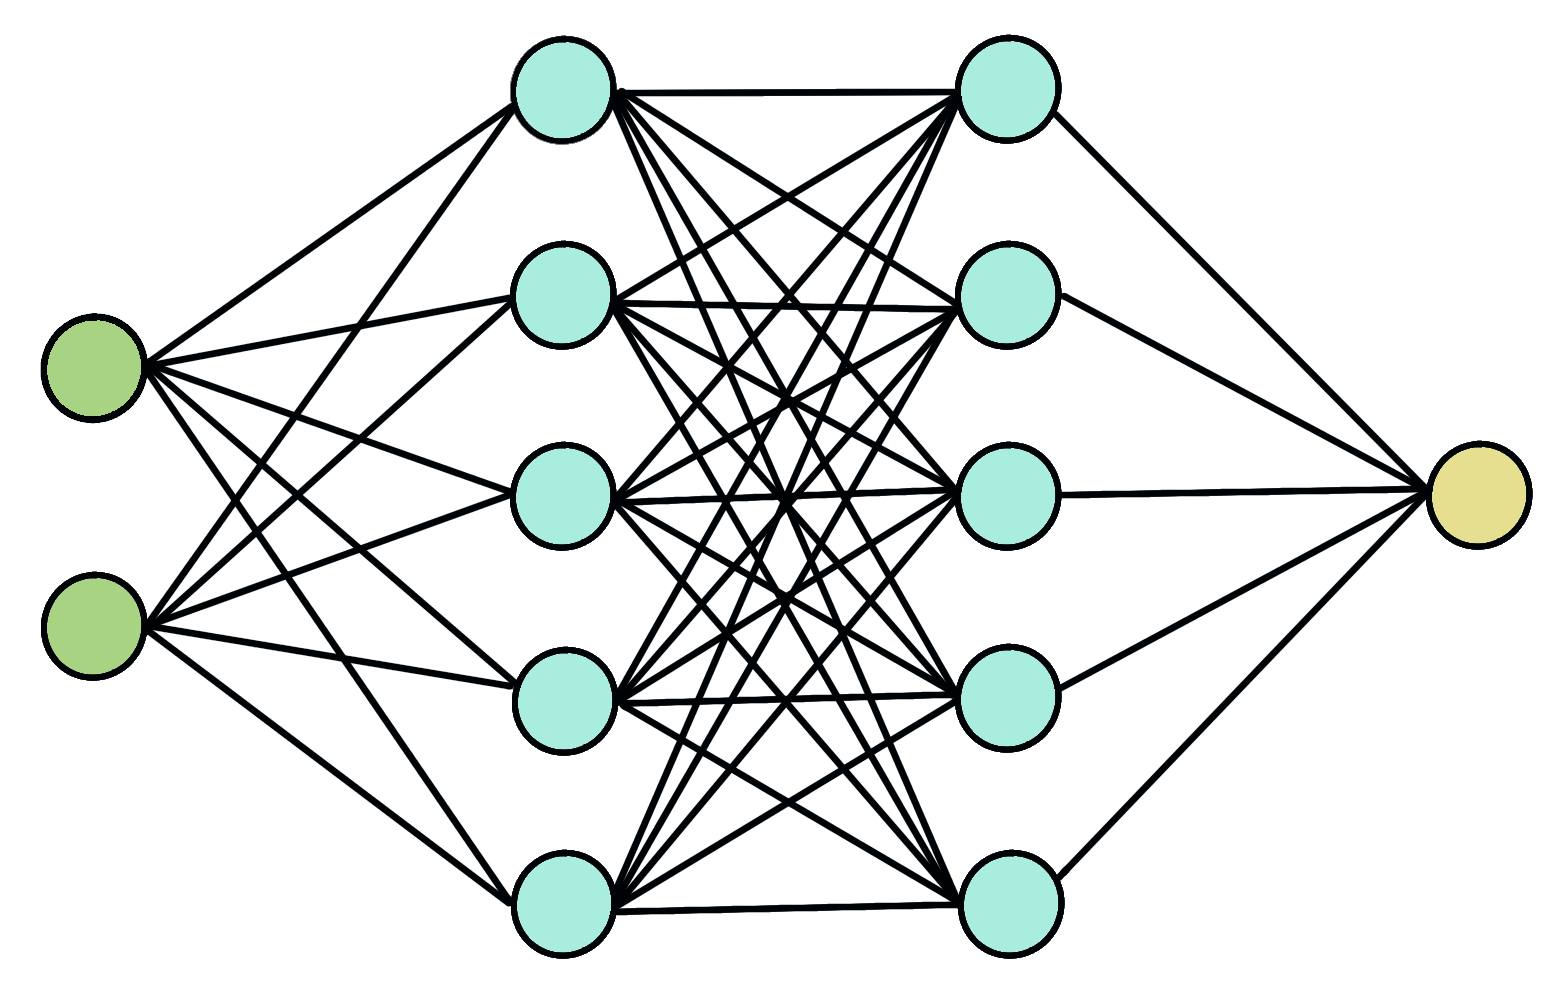
\includegraphics[width=2.8cm]{network.png}};
            \draw[->, black, line width=2pt] (6.75,1.25) -- (7.75,1.25);

            \draw[draw=black,dashed] (8,0) rectangle ++ (5,2.5);
            \node at (10.5,1.85) {\Large \textbf{PINN evaluation}};
            \node at (10.5,1.1) {\large $u_\theta$ : prediction for};
            \node at (10.5,0.5) {\large the parameter $\mu$};

            \draw[->, black, line width=2pt] (13.25,1.25) -- (14.25,1.25);
            \node at (15.40,0.25) {\large \textbf{FEM solver}};
            \node at (15.40,-0.25) {\large \textbf{enriched by $u_{\theta}$}};
            \node[draw=none, inner sep=0pt] at (15.4,1.5) {
\includegraphics[width=2cm]{FEM.png}};
            \draw[->, black, line width=2pt] (16.5,1.25) -- (17.5,1.25);

            \draw[draw=black,dashed] (17.75,0) rectangle ++ (6,2.5);	
            \node at (20.75,1.85) {\Large \textbf{Output}};
            \node at (20.75,1.1) {\large enriched FEM solution};
            \node at (20.75,0.5) {\large (depending on the mesh size $h$)};

            % \node[draw=black,dashed,align=center,yshift=-2em,text width=11.5em,minimum height=8em] at (20,1.85) {
            % \Large \textbf{Output:} \\[.20em]
            %             \large enriched FEM solution \\[.00em]
            % };
        \end{tikzpicture}
    \end{tcolorbox}
\end{document}
